\documentclass{report}

\usepackage{amsmath}
\usepackage{amssymb}
\usepackage{appendix}
\usepackage{biblatex}
\usepackage{booktabs}
\usepackage{caption}
\usepackage{changepage}
\usepackage{float}
\usepackage{graphicx} % Required for inserting images
\usepackage{lipsum}
\usepackage{listings}
\usepackage{minted}
\usepackage{multirow}
\usepackage{pgfplots}
\usepackage{setspace}
\usepackage{tocbibind}
\usepackage{todonotes}
\usepackage[a4paper,margin=1in]{geometry}

\lstset{
  basicstyle=\ttfamily\small,
  breaklines=true,
  frame=single
}

\captionsetup[lstlisting]{%
  labelformat=empty,  % no “Listing X.Y” label
  labelsep=none       % no extra colon or dash
}

\addbibresource{references.bib}

\title{Automated Demographic Segmentation and Sentiment Analysis using LLMs}
\author{Conrad Khakhria}
\date{November 2024}

\setlength{\parindent}{0pt}
\setlength{\parskip}{1em} % Adjust '1em' to your desired gap size

\onehalfspacing


\begin{document}

\maketitle

\begin{abstract}
This thesis investigates the use of large language models (LLMs) for consumer trend prediction across demographically-segmented social media data. This is motivated by the ability of LLMs to process, reason about, and draw detailed conclusions about vast amounts of complex, unstructured text data. This thesis attempts to determine therefore whether LLMs are able to determine new consumer trends from social media posts while automatically deducing which demographic segments the users who made each post belongs to.

The subject of this thesis naturally divides the research into two categories: that of automated demographic segmentation, and that of consumer trend prediction. Although the data used for each component will be the same (i.e. unsegmented text-based social media posts), the methodology for each will be profoundly different. Demographic segmentation is a well-explored area of research and industry practice, and the performance of a machine learning-based approach is easily evaluated as vast amounts of rich, labelled demographic data is readily available. For example, the \textit{Sentiment140}dataset consists of 1.6 million tweets, each with demographic segment labels. Standard evaluation methods for machine learning classification algorithms can be used with data like this to directly evaluate the performance of LLM-based demographic segmentation. Trend prediction, on the other hand, is less straightforward: predictions of consumer trends are most valuable when they are novel, and the novelty and usefulness for business applications of a consumer trend prediction cannot be evaluated with statistical error metrics. An analysis of the results of trend predictions by LLMs will be by nature qualitative.

The thesis consists of three investigations, each original investigations into new LLM-based approaches problems in business analytics. The research strucutre will be as follows:

\begin{enumerate}
    \item \textbf{Experiment 1: Automated Demographic Segmentation}

    This study makes a hypothesis about the efficacy of an LLM-based approach to demographic segmentation. This hypothesis is evaluated by comparing the performance of this approach to other existing approaches (relative performance), as well as directly presenting the results of this approach against datasets of segmented social media post data (absolute performance).

    \item \textbf{Experiment 2: Large Language Model Historical Consumer Trend Prediction}

    This study directly tests the ability of large language models to predict consumer trends using segmented social media post data. The experiment will be conducted using historical social media post data, which the large language models will use to 'predict' the historical consumer trend.

    \item \textbf{Experiment 3: Application of LLM-segmented Consumer Trend Prediction to Current Social Media Data}

    This study will apply the models used in experiments 1 \& 2 to current social media post data. This will produce a prediction of a future consumer trend.
\end{enumerate}

This thesis presents the following original contributions to science:

\begin{itemize}
    \item  Given how new large language models are as a technology, little research has been conducted into the ability of LLMs to conduct demographic segmentation. Experiment 1 provides empirical data on how accurately LLMs can infer demographic information on social media data, and an effective LLM-based approach will be able to generate a vast amount of labelled demographic segment data from social media posts.

    \item There is currently very little research into the effectiveness of machine learning-based approaches to consumer trend prediction, in particular LLM-based approaches. Experiment 2 will provide one of the earliest formal investigations into this approach.

    \item There is debate among researchers about the ability of LLMs to generate novel ideas, and in particular whether they have the ability to outpace humans in this regard. Experiment 2 directly investigates this question, and in particular with a focus on deriving both novel and useful conclusions from a specific set of unstructured text data.
\end{itemize}
\end{abstract}

\tableofcontents


\chapter{Introduction}

\begin{adjustwidth}{0.5in}{0.5in}
    \textit{This chapter presents an overview of the thesis by discussing the motivation behind the research problem, as well as its objectives, experiments, and structure. The chapter begins with information on demographic segmentation and consumer trend prediction, an appraisal of their importance for businesses who sell consumer goods, and a brief discussion of the state-of-the-art in the field with reference to machine learning. The chapter then outlines the research objectives, experiments, scientific contributions, and structure of the thesis.}
\end{adjustwidth}

\section{Motivation}

\begin{itemize}
    \item Analytics from social media are one of the most widely and effectively utilised sources of information available, with data like watch time, click-through rates, think of better examples, being some of the most valuable resources provided by social media platforms. These data are used heavily for marketing and product development, among many other things

    \item However, it has so far proven largely infeasible to derive more complex conclusions from social media post data itself: text data from social media has little structure, and is highly contextual, requiring a great deal of knowledge of the external world.
    
    \item As such, social media post data is in many ways an untapped resource: with enormous numbers of peoples thoughts and opinions being publicly broadcast constantly, social media posts contain a wealth of information about consumer trends, with the bottle-neck so far being the ability to process this information.

    \item LLMs can process huge amounts of unstructured text data, drawing on their own knowledge to infer complex conclusions about text. Examples include RAG, LLM web search, and I guess stuff like code generation/debugging (cite a code debugging thing)

    \item LLMs are therefore a game-changer: with their ability to instantly reason about, summarise, and answer questions about huge amounts of text data, they are so far the most promising potential approach in utilising the resource that is social media post data for gathering consumer information in real-time and at scale.

    \item The prediction of consumer trends is of course vital to the continued growth and development of any business: maybe we can give an example of money lost by a company that wasn't able to predict an upcoming trend. Furthermore, for very large businesses operating across multiple continents, a deep understanding of shifts across specific demographic groups is necessary.

    \item LLMs may be able to assist with both of the above:

    \begin{enumerate}
        \item Obtaining accurate demographic information from social media post data is not always possible, and in many cases, the specific information that a company needs may not be directly recorded. LLMs show promise in complex reading comprehension tasks, drawing on large amounts of prior knowledge, and may be able to infer demographic information from social media posts. This will allow companies to have access to demographic information at a lower cost, and potentially allows for the inference of demographic characteristics that are otherwise not recorded.

        \item LLMs can process text data at a level that is incomparable with that of humans. Combining this with their increasing ability to perform very well in reading comprehension tasks suggests that they may be able to effectively infer upcoming consumer trends from social media data. This 
    \end{enumerate}
\end{itemize}

\section{Research Objectives}

\begin{itemize}
    \item The main objective of this research is to determine whether large language models can be used to significantly improve upon existing techniques for consumer trend prediction, providing faster and more in-depth insights into upcoming consumer trends.

    \item Whereas existing ML approaches have a strong ability to predict consumer behaviour in a classification setting, this is very narrow, limited to selecting between pre-defined options expressed in the classification/regression setting (check that this is true but it seems obvious)

    \item This research therefore evaluates the ability of large language models to produce not just accurate but also novel, and open-ended, insights into future consumer trends. We will compare how they perform against traditional algorithms used in both supervised and unsupervised learning problems, as they apply to future consumer trend prediction

    \item This research also attempts to use LLMs for the inference of demographic characteristics from social media posts. This would allow for the prediction of future consumer trends across an incredibly fine-grained range of different demographic groups, without the possible limitation of either data quality or range of demographic characteristics actively recorded by social media platforms.

    \item This study therefore both compares LLMs to traditional methods for inference of demographic information from social media data, as well as establishing whether they can infer these data in greater detail or to a wider range of characteristics than is otherwise currently possible
    
\end{itemize}

\section{Experiments}

\begin{enumerate}
    \item Automated demographic segmentation.

    \begin{itemize}
        \item The first experiment aims to observe whether LLMs can infer demographic characteristics, e.g. age, sex, location, about posters from their social media posts.
    
        \item This is original research: existing research into demographic inference with AI focuses on much more narrow settings, for example "Customer profiling, segmentation, and sales prediction using AI in direct marketing" which uses unsupervised learning for categorisation (thus unlabelled) and boosting trees for classification (thus less rich).
    
        \item This experiment treats demographic segmentation as a classifiaction problem, comparing LLMs to traditioanl classification algorithms. We will compare the capabilities of LLMs, handling largely un-preprocessed data, to those of the traditional algorithms such as the SVM and boosting and basic deep learning, combined with techniques from 'classical' NLP such as TF-IDF.
    \end{itemize}





    \item Large language model historical consumer trend prediction.

    \begin{itemize}
        \item This study investigates whether LLMs can predict future consumer trends, across different demographics, from demographically-segmented social media post data.

        \item Although there is a wide body of research in predicting consumer trends using more traditional approaches in machine learning, this is the first research I am aware of that attempts to do this with LLMs using social media data.

        \item Where existing research applies ML in comparatively simpler settings, such as time series forecasting for sales, this research leverages the unique potential of LLMs to produce novel output outside of a given structure. This means that, in principle, we will be able not just to extrapolate existing trends or sales volume for existing products, but identify consumer behaviour and desires for entirely new kinds of products and services.
    \end{itemize}


    \item Application of LLM-segmented consumer trend prediction to current soical media data


    \begin{itemize}
        \item This study combines the approaches from the previous two experiments and applies them to current social media data, attempting to predict an actual future consumer trend.

        \item This experiment will produce results which, unconventionally, cannot be directly evaluated at this time. Although the methodology will have been evaluated in the previous two sections, the predictions produced from current social media data can only be assessed in the future.

        \item The primary focus of this experiment is to provide a real-world example of how a consumer trend prediction by an LLM would look, outside of a contrived research setting.
        
    \end{itemize}

\end{enumerate}

\section{Scientific Contributions}

This work contributes to existing research across multiple fields in the following ways:


\begin{enumerate}
    \item Comparison of LLM-based approaches to traditional methods in natural langauge processing (NLP). The first part of this research applies LLMs to a classification problem, in the form of demographic segmentation, where it is directly benchmarked against more traditional approaches in ML classification and NLP. The performance of each approach will be compared directly with standard classification metrics such as accuracy, precision, recall, and f1 score. 

    \item Empirically evaluates LLM performance in complex reading comprehension tasks. Both the demographic segmentation and consumer trend prediction are, ultimately, complex reading comprehension tasks. This research therefore provides insight into the ability of LLMs to derive complex insights from potentially information-sparse data.

    \item Establishes a new approach to consumer trend prediction. Traditional approaches to consumer trend prediction rely heavily on human insight, either in the form of direct human interpretation of written information, or carefully hand-crafted features when machine learning approaches are employed. This new approach to consumer trend prediction is therefore significantly more scalable, potentially eliminating the need for human work in general. Furthermore, this approach may combine the predictive accuracy of machine learning approaches with the unstructured open-endedness of human interpretation.

    \item Direct empirical study into the ability of LLMs to produce novel conlusions. LLMs are a relatively new technology, and there is significant academic debate about whether they are able to derive novel conclusions, across a range of different settings. The latter part of this dissertation addresses this question directly, with LLMs being tasked with deriving future consumer trends in a conceptual, rather than numerical, setting.

    \item Advances the currently thin existing research into LLM temporal event forecasting. \todo{finish}

    \item Produces an original and current prediction of a future consumer trend. The third empirical investigation in this dissertation applies the techniques evaluated in the previous two to current social media data, with the aim of producing a real prediction of a future consumer trend. \todo{as far as I can tell} There are no consumer trend predictions generated in this way in academic literature, and this will therefore provide an important result which can be evaluated in the future.
\end{enumerate}

\section{Thesis Structure}

This thesis is organised as follows:

\begin{itemize}
    \item \textbf{Chapter 2: Background and Literature Review}

    Relevant academic literature about both related research as well as the underlying technological and conceptual underpinnings of this thesis are reviewed, providing the background necessary for understanding this research. This includes an introduction to supervised and unsupervised machine learning, generative machine learning, as well as LLMs themselves. A review of literature in social media data mining is also presented. Furthermore, this section also reviews existing research into demographic segemntation and consumer trend prediction, both with 'manual' and machine learning-based approaches.

    \item \textbf{Chapter 3: Automated Demographic Segmentation}

    This chapter provides a direct evaluation of the ability of LLMs to infer demographic characteristics from social media post data. This experiment is treated as a classification problem, and the LLMs are directly benchmarked against traditional machine learning approaches to classification in NLP problems. Standard classification metrics such as accuracy, precision, recall, and f1 score are used to evaluate the performance of the LLM-based approach.

    \item \textbf{Chapter 4: Large Language Model Historical Consumer Trend Prediction}

    This experiment evaluates whether LLMs can predict 'future' consumer trends from social media data. A historical consumer trend is chosen, and social media data from up to the time that this trend manifests is given to an LLM as input for predicting the trend. In this study, the LLM is tasked both with predicting all future consumer trends indicated by the social media data, as well as being asked directly whether the social media data it encounters suggests that the specific consumer trend is likely to develop.

    \item \textbf{Chapter 5: Application of LLM-segmented Consumer Trend Prediction to Current Social Media Data}

    This study combines the approaches used in both chapters 3 and 4, applying LLMs to current, unlabelled social media post data to predict actual future consumer trends across different inferred demographic groups. The results of this study are directed towards an actual future event, and therefore cannot immediately be directly evaluated. However, this section does contain a detailed comparison of results obtained using different language models, as well as data from different social media platforms and sub-groups therein.

    \item \textbf{Chapter 6: Conclusion and Future Work}

    The final chapter of this thesis provides an overall conclusion of this research, summarising and interpreting the results obtained. This is followed by recommendations of future research to be undertaken following this.

\end{itemize}




\chapter{Background and Literature Review} \label{sec:lit-review}

\begin{adjustwidth}{0.5in}{0.5in}
    \textit{This chapter presents background information relevant to the thesis, both in terms of the subjects of the research and the methodology that will be employed. In particular, the first part of this chapter will present the state of existing research and practice in both demographic segementation (automated and manual) as well as consumer trend prediction, and the second will give a broad overview of machine learning, in particular large language models and data mining.}
\end{adjustwidth}

This thesis consists of three experiments, with the final experiment being largely derived in methodology from the first two. Each of the experiments share a significant knowledge base (in particular, that of LLMs and social media data-mining), but there are a range of significant differences, in particular in terms of the problem setting. 

The first part of this chapter outlines the technologies and concepts that are fundamental both to much of the existing research that follows in this literature review as well as to this thesis' own experiments. It begins with an introduction to machine learning, in particular the distinction between supervised and unsupervised learning, continues onto LLMs, and then explains the metrics that will be used for evaluating these machine learning models. The section concludes with a detailed treatment of social media data-mining.

\todo[inline]{consider whether to remove the bit about data mining considering that I'm using pre-built datasets}

The second part of this chapter is the \textit{Application Domain} section, which explores the state of the art in algorithmic and data-driven demographic segmentation and consumer trend prediction.


\todo[inline]{give a broad and brief overview of the state of the art in both demographic segmentation and consumer trend prediction}
\todo[inline]{talk about how each expt contains a mini lit review}


\section{Method Development}

This section discusses the fundmentals of supervised and unsupervised learning, covering fundamental algorithms such as linear regression and decision trees. It then goes into depth on concepts in natural language processing, and in particular large language models. Following this is an overview of the evaluation metrics that will be used for the first experiment of this thesis, which is in the classification setting. [also maybe data mining].

\subsection{Machine Learning}

\subsubsection{Supervised and Unsupervised Learning}

\begin{itemize}
    \item There are three types of machine learning: supervised, unsupervised, and reinforcement. Relevant to this dissertation are supervised and unsupervised learning.

    \item Supervised learning problems are ones in which 'input' data points, or \textit{features}, are provided with corresponding 'output' data points, or \textit{labels}, and the algorithm is tasked with creating a model which can predict the label for novel data points that it has not yet encountered. These labels can either be continues values, in the \textit{regression} setting, or discrete, in the \textit{classification} setting.

    \item A classic supervised learning problem is with the MNIST dataset, a set of 70,000 hand-written digits commonly used as a benchmark for image recognition \cite{lecun1998gradient}.

    \item This dissertation focuses primarily on classification problems, rather than regression. Linear regression will be briefly introduced, primarily to motivate logistic regression, a simple binary classification algorithm.

    \item Unsupervised learning problems, in contrast, provide only features, and algorithms are tasked with detecting patterns within the data. Two common types of unsupervised learning algorithm are \textit{dimensionality reduction}, in which they select the most 'important' components of the data points in a dataset, or \textit{clustering}, in which they determine distinct groupings of points in a dataset, either of a specified number or not.

    \item Following the supervised learning algorithms presented in this section will be a number of fundamental unsupervised learning algorithms, both dimensionality reduction and clustering.
    
\end{itemize}

\subsubsection{Linear Regression}

\begin{itemize}
    \item Linear regression, and in particular least-squares regression, is the most studied family of regression models in statistics and machine learning. Least-squares linear regression models attempt to find a linear function $f(x) = w \cdot x + b$ to predict labels $y$ from input features $x$ by minimising the \textit{residual sum of squares} (RSS) loss function between predicted labels $f(x_i)$ and true values $y_i$: 
    \begin{align}
        f^* &= \arg\min_f \sum_{i=1}^N \left( y_i - f(x_i) \right)^2. \notag \\
        &= \arg\min_{w, b} \sum_{i=1}^N (y_i - w \cdot x_i - b)^2, \label{eq:ols-rss-error}
    \end{align}

    \item (by convention, $x_i$ is often considered to contain a constant dimension always equal to $1$, thus allowing the $b$ parameter to be included in $w$. Thus, $f(x_i) = w \cdot x_i$).

    \item There are multiple ways to find the optimal model $f^*$. For example, in \textit{ordinary least-squares} regression, admits the following analytical solution:
    \begin{equation}
        w = (\textbf{X}^\top \textbf{X})^{-1} \textbf{X}^\top y,
    \end{equation}
    where $\textbf{X}$ is the \textit{design matrix} whose rows are the input vectors and $y$ is the output vector whose elements are the corresponding labels.

    \item More common is the use of numerical methods, and in particular gradient methods, for efficiently obtaining a well-performing model $w$. A gradient method-based approach to optimising a least-squares linear model will, from some starting point $w_0$, change the parameter iteratively in the direction that causes the RSS error to decrease as quickly as possible, either for a fixed number of iterations or until the method has converged on or close to a minimum possible error.

\end{itemize}


\subsubsection{Logistic Regression}

\begin{itemize}
    \item Logistic Regression adapts linear regression models to the task of binary classification, i.e. classification where the labels can take on one of exactly two possible values. This is achieved by passing the output of a normal linear regression model through a \textit{logistic unit} (logit) function $\sigma$, which 'squeezes' it to be between $0$ and $1$:
    \begin{equation}
        f(x) = \sigma(w \cdot x)
    \end{equation}
    The classification is taken to be whichever of the two extremities the prediction is closest to.

    \item The most common logit function is the \textit{logistic sigmoid} function:
    \begin{equation}
        \sigma(z) = \frac{1}{1 + e^{-z}},
    \end{equation}
    which constrains values $z \in \mathbb{R}$ as follows:

    \begin{center}
    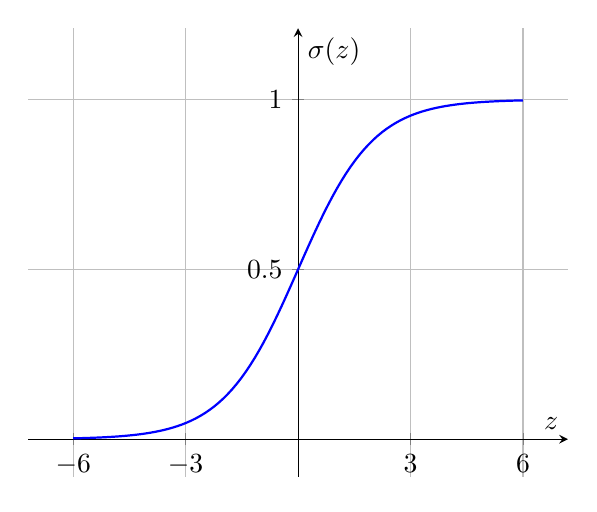
\begin{tikzpicture}
        \begin{axis}[
            axis lines = middle,
            xlabel = {$z$},
            ylabel = {$\sigma(z)$},
            samples = 100,
            domain = -6:6,
            ymin = 0, ymax = 1.1,
            enlargelimits=true,
            xtick={-6,-3,0,3,6},
            ytick={0,0.5,1},
            grid = major
        ]
            \addplot [blue, thick] {1/(1 + exp(-x))};
        \end{axis}
    \end{tikzpicture}
    \end{center}

    With this function, distance from 0 can be understood as being analagous to 'certainty' that a particular value $x$ is firmly categorised as either 0 or 1. In particular, the logistic sigmoid function $\sigma(z)$ represents the \textit{probability} that $z$ is categorised as 1 rather than 0:
    \begin{equation}
        \sigma(w \cdot x) = P(y=1 \; | \; x).
    \end{equation}
    
    \item Given that this probability is defined in terms of the linear function $w \cdot x$, we get that the line $w \cdot x = 0$ itself represents the set of points $x$ for which the probability of classification $y=1$ is exactly $\frac{1}{2}$. This is known as the \textit{decision boundary}, and the prediction made by a logistic regression model is effectively given by which side of the decision boundary a point $\sigma(w \cdot x_i)$ falls on.

    \item Logistic regression models are optimised differently to normal linear regression models, on account of the non-linear logit function. A common approach is via Maximum Likelihood Estimation (MLE), which by taking the log-likelihood leads to the following loss function:
    \begin{equation}
        \mathcal{L}(x, y \;;\; w) = -\sum_{i=1}^N [y_i \log(\sigma(w \cdot x_i)) + (1-y_i) \log(\sigma (w \cdot x_i))].
    \end{equation}
    Unlike OLS regression, this loss function does not admit a closed-form analytical solution. It is however convex, and thus can be optimised using gradient descent with respect to $w$.

\end{itemize}

\subsubsection{Kernelised SVM and Decision Trees} \label{sec:lr-svm-decision-trees}

\begin{itemize}
    \item The previous examples have been of algorithms that use a linear model. In the regression setting, this means that the data is assumed to follow a linear trend, and in the binary classifications setting it assumes that the two categories of data can be separated with a linear decision boundary. The following presents two significantly different approaches to classification of non-linear data.

    \item The Support Vector Machine (SVM) is a binary classification algorithm which, similarly to logistic regression, fits a linear decision boundary $w \cdot x_i + b = 0$ between two categories of data. This algorithm is distinguished from least-squares based regression/classification approaches in terms of the loss function that it uses for fitting this line (or hyperplane, in multiple dimensions): instead of minimising the RSS loss, an SVM model is optimised by maximising the \textit{margin}, that is, the distance between the actual data points and the discriminant boundary, with the constraints that the points must correctly classified, i.e. on the right side of the distcriminant boundary.

    \item This maximisation problem results in this loss function:
    \begin{equation}
        \mathcal{L}(x, y \; ; \; w, b) = \frac{1}{2} \|w \|^2 + C \sum_{i=1}^N \xi_i,
    \end{equation}

    where $C$ controls the trade-off between maximising the margin and allowing for mis-classifications, and $\xi_i = \max(0, 1 - y_i (w \cdot x_i + b))$ is the \textit{hinge loss}, which grows with distance from the margin only if a point $x_i$ is classified on the incorrect side of the discriminant boundary:

    \begin{center}
    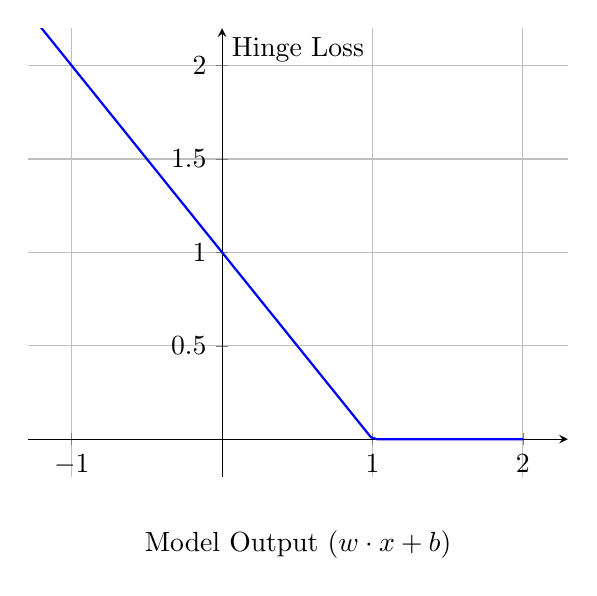
\begin{tikzpicture}
        \begin{axis}[
            axis lines = middle,
            xlabel = {Model Output ($w \cdot x + b$)},
            xlabel style={at={(axis description cs:0.5,-0.1)}, anchor=north}, % Moves xlabel below the axis
            ylabel = {Hinge Loss},
            samples = 100,
            domain = -2:2,
            ymin = 0, ymax = 2,
            enlargelimits=true,
            xtick={-2,-1,0,1,2},
            ytick={0,0.5,1,1.5,2},
            grid = major,
            legend pos=north east
        ]
            % Hinge loss for y = 1
            \addplot [blue, thick] {max(0, 1 - x)};
        \end{axis}
    \end{tikzpicture}
    \end{center}

    \item The SVM can be adapted to non-linear data by expressing the algorithm with a \textit{kernel}, which is an inner product $\kappa (x_i, x_j)$ between two input points $x_i$ and $x_j$ which implicitly maps them into a new feature space to create a non-linear discriminant boundary. For example, a quadratic discriminant boundary can be obtained with the kernel
    \begin{align}
        \kappa(x_i, x_j) &= (x_i \cdot x_j + 1)^2 \notag \\
        &= (x_i \cdot x_j)^2 + 2(x_i \cdot x_j) + 1.
    \end{align}

    Common kernels include:
    \begin{enumerate}
        \item \textbf{Linear Kernel:} $\kappa(x_i, x_j) = x_i \cdot x_j$ (Equivalent to linear SVM)
        \item \textbf{Polynomial Kernel:} $\kappa(x_i, x_j) = (x_i \cdot x_j + c)^d$ (which will fit to polynomials of degree $d$)
        \item \textbf{Radial Basis Function (RBF) Kernel:} $\kappa(x_i, x_j) = \exp\left(-\gamma \|x_i - x_j\|^2\right)$
        \item \textbf{Sigmoid Kernel:} $\kappa(x_i, x_j) = \tanh(\alpha x_i \cdot x_j + c)$
    \end{enumerate}

    The RBF kernel is of particular interest, as it is a \textit{universal approximator}, i.e. it is capable of approximating any function \cite{wang2004svm-universal-approximator}. This is because it implicitly maps data points into an infinite-dimensional feature space, meaning that the RBF-kernelised SVM can fit a discriminant boundary to any continuous function.

    \todo[inline]{check if this is a correct use of 'universal approximator'}

    \item Decision tree learning is a paradigm of machine learning which is distinct from linear methods like least-squares regression or the SVM. Instead of fitting a linear function to either approximate a continuous function or decide between two categories of discrete labels, decision tree learning algorithms build a tree where nodes represent discriminants between different sections of the input space and leaves contain predictions of the corresponding label values.

    \item The most commonly used decision tree algorithm is the Classification and Regression Tree (CART), which recursively partitions the input space into sections and then assigns a prediction to each section by taking the mode of all data points $y_i$ within it. In particular, at each iteration a partition is divided into two sub-partitions, i.e. children of the partition's node in the tree, by choosing the split that minimises the \textit{Gini impurity}, a measure of how often a randomly chosen sample from within a partition would be misclassified if it were to be assigned a random label.  

    \item CART learning is capable of producing accurate approximations of non-linear functions in both the regression and classification setting, and is one of the most widely used machine learning techniques that doesn't use linear models.
\end{itemize}

\subsubsection{Multiclass Classification} \label{seec:lr-multiclass}


\subsubsection{Deep Learning}


\subsubsection{[Weird stuff like self-supervised and generative]}






\subsection{Natural language processing and Large Language Models}

\subsubsection{Fundamentals of NLP}

\subsubsection{Early NLP approaches}

\subsubsection{The Transformer Architecture and LLMs}





\subsection{Model Evaluation} \label{sec:lr-model-evaluation-selection}

\subsubsection{Classification Evaluation Metrics}

\subsubsection{Evaluation Metrics for NLP and LLMs}

\subsubsection{Model Selection}


\subsection{Social Media Data Mining}


\section{Application Domain}

\subsection{Demographic Segmentation}

\subsection{Consumer Trend Prediction}




\chapter{Automated Demographic Segmentation}

\begin{adjustwidth}{0.5in}{0.5in}
    \textit{This study presents an empirical means of automating demographic segmentation from social media data using large language models. The study adapts existing techniques for use with the kinds of unstructured data that social media posts and profiles present, and compares the effectiveness of LLM-based approaches to existing techniques. This chapter discusses the data set used for the experiment, the setup of the experiment itself, and the results that it yielded.}
\end{adjustwidth}


\section{Introduction}

\begin{itemize}
    \item Accurate demographic information is vital to localising consumer trend forecasts to different demographic groups. Having an accurate model for how consumer trends may change between different groups allows for
    \begin{enumerate}
        \item Better targeting of advertising

        \item Development of new product categories, across different markets

        \item Forecasting demand for existing product categories
    \end{enumerate}

    \item Companies with a particular broad range of products and markets require a particularly rich set of demographic indicators to capture information about their consumers. Attempts to infer consumer trends from social media, for example, must therefore robustly distinguish these consumer trends as they apply to different consumer groups.

    \item However, accurate or complete demographic information is hard to come by for social media posts, for a variety of reasons. For example, many social media users will not publicly display their demographic information: in particular, some social media sites such as Reddit have a stronger culture of anonymity than sites like Facebook, with usernames or bios not necessarily being linked to actual information about the users \cite{reddit-pseudoanonymous}. Furthermore, even when demographic information can be obtained directly, it may be insufficiently precise or not cover desired categories, such as income group or nationality. For these reasons, demographic inference may be preferable, as it allows for the collection of demographic information without limits on categorisation, specificity, or completeness.

    \item LLMs are a potentially promising approach to inferring demographic information from social media data, given their ability both to apply vast amounts of pre-existing knowledge to data as well as to make inferences about the language. In particular, LLMs are able to solve problems, including in a classification setting, posed in natural language with little to no training data. This means that, in principle, LLMs could be used to segemnt people by any desired consumer group, regardless of category or specificity, without the need to obtain potentially unfeasibly large amounts of training data, allowing for vastly increased flexibility in segmentation for consumer trends.

    \item Much work has already been done in the use of LLMs for demographic inference, as discussed in the bibliography, \todo{Do this ofc.} using a variety of different datasets and data types. Recent advances in multimodal LLMs for example have allowed for profile pictures and other image data to be used in enhancing demographic predictions. 

    \item To determine whether automated LLM-based demographic segementation of social media posts is viable or represents a meaningful improvement over other common techniques, it is imperative to observe directly how LLMs compare to traditional NLP approaches. This experiment aims to produce an empirical comparison of LLM-based approaches to demographic inference to established techniques in machine learning NLP classification, evaluating the performance of each approach with standard classification evaluation metrics.
\end{itemize}

\section{Data Set}

\subsection{Data Set Choice}

\begin{itemize}

    \item This experiment required a large body of social media text posts, annotated with demographic labels.

    \item This presents two challenges. First of all, due to increased concerns about privacy and significant regulation on data protection, there are few easily-accessible datasets of demographically-labelled social media posts. This applies in particular to social media data from after 2018, when GDPR came into effect.

    \item The second problem is perhaps more fundamental: as discussed earlier, even if people openly present demographic information about themselves, it is inherently difficult to verify whether this information is accurate. Most existing datasets of demographically-labelled social media data either use self-reported or inferred demographic labels, and thus it is difficult to know whether these labels are accurate.

    \item As this first experiment is intended to benchmark the ability of LLMs to infer demographic information, a dataset would need to fit three criteria:

    \item The analysis is conducted on the \textit{Blog Authorship Corpus} (BAC), a collection of 681,288 blog posts written on or before 2004\cite{blog-authorship-corpus}. The BAC is a well-established dataset which consists of text-based blog posts annotated with self-reported age and gender.

    \item This is the best dataset for our purposes for four reasons:
    \begin{enumerate}
        \item It is freely available and well-established, with much prior research in demographic inference over the past 20 years using it. This means that, in addition to the model comparison that we can derive from our experiment, we can compare our LLM-based approach directly to a broad range of cutting-edge approaches.

        \item The demographic labels are relatively-reliable: although it is possible that some of the blog's self-reported age and gender will be erroneous, it is still more useful for benchmarking prediction than either synthetic social media data or datasets with inferred demographic labels.

        \item The dataset is roughly well-balanced. In particular, each blog post is in one of roughly three age-ranges: teenagers aged 13-17, of which there are 8,240, young adults aged 23-27, of which there are 8,806 posts, and adults aged 33-47 of which there are 2,994. In each age group there are exactly the same number of men and women

        \item The dataset contains both numeric and categorical data, with age being supplied as a number and gender being either ``male" or ``female". This means the experiment will be able to evaluate the LLMs in both a classification and a regression setting. 
    \end{enumerate}

    \item The primary issue with the BAC is its age: given that it consists of blog posts from over 20 years ago, social media usage styles will have changed significantly since the time that the posts were collected. This could mean that, applied to contemporary social media data, the LLM approach could perform significantly better or worse, depending on how differently people of different demographic groups may express themselves now and how many examples of these new stylistic demographic expressions were in the LLM's training data.

    \item The \textit{PAN Author Profiling datasets} are collections of Twitter (now X) posts for each year starting in 2013, across different languages, with demographic labels including age and gender \cite{PAN-age-gender-2013}. These datasets address the issue with recency, but as they exclusively use Tweets, the dataset consists purely of short-form rather than longer-form content—in particular, examples in the dataset are limited to being up to 140 characters. This means that the results of this study, had we used the \textit{PAN Author Profiling datasets}, would be less representative of performance on other social media platforms like Reddit where significantly longer posts are more common.
\end{itemize}

\subsection{Data Preprocessing}

\begin{itemize}
    \item The \textit{Blog Authorship Corpus} consists of purely text-based blog posts with self-reported annotations for age, gender, employment sector, and star sign. Only the first two of these demographic categories were included, as the dataset doesn't contain fully representative and balanced examples for employment sector and because horoscopes are less useful predictors of behaviour than age and gender.

    \item The gender labels consist exclusively of the strings ``male" and ``female", and were thus left unmodified. 
    
    \item Although age is recorded as an integer, the standard approach to age classification in academic literature \todo{find a source} is to group the ages into ``buckets", and then treat these as a classification target. For this reason, numeric ages were turned into 5-year age ranges (e.g. 24 became '20-25', etc).
\end{itemize}

\section{Experiment}

\begin{itemize}
    \item This experiment is effectively a standard classification problem for both age and gender. This means that the performance of the LLM can be compared directly against that of standard NLP classification  techniques.

    \item To provide a benchmark, this experiment uses standard shallow NLP approaches \todo{find some source for why these are standard}: in particular, we use three algorithms which broadly represent the most commonly used families of algorithms used in shallow supervised learning:

    \begin{enumerate}
        \item \textbf{Least-Squares Linear Regression}

        Least-squares linear regression models are the most commonly used machine learning models. They are generally fast to train and provide a strong baseline for comparison.

        We use logistic regression, which adapts least-squares regression to the binary classification setting. This is extended to multiclass classification (for predicting different age brackets) using the one-versus-rest strategy, as discussed in section \ref{seec:lr-multiclass}.

        \item \textbf{Support Vector Machine}

        Support Vector Machine models are another type of linear model, as discussed previously in Section \ref{sec:lr-svm-decision-trees}, which are trained by solving a different optimisation problem to least-squares models. They are often more robust to overfitting than least-squares linear models, and the kernel allows them to fit to highly non-linear decision boundaries.

        In the classification setting we use one-versus-one Support Vector Classification.

        \item \textbf{Random Forest}

        Random forest is a non-linear ensemble method, which distinguishes it from the previous two approaches. It provides a meaningful point of comparison, as random forest models can perform significantly differently to linear models, whether they're kernelised or not.

        In particular we use CART, which can handle multi-class classification natively.
    \end{enumerate}

    \todo{explain why we're using different multiclass strats for SVM and LR}
    
    \item These algorithms are adapted for use in an NLP setting with a vectoriser, which transforms arbitrary-length text data into fixed-length vector representations of the different words that appear in the text, which is a standard and well-studied (though comparatively simplistic) approach to NLP in classification and regression contexts.

    \item Applying LLMs to a classification task is less straightforward, and the flexibility that comes with their prior knowledge and ability to generate arbitrary-length text comes at the cost of associated complexity when generating certain kinds of outputs. Any approach must fundamentally involve taking text as input and producing categorical predictions for age and gender as output. Although many larger models can now be forced to produce output with a given output structure, many models, and in particular smaller ones, will require more elaborate prompt engineering \todo{determine whether 'prompt engineering' is something you'd actually say} instead.

    \item For this experiment, two kinds of prompt engineering were required. First of all, the model was given explicit instructions to follow a given output JSON schema, and was given precise instructions as to the kinds of output it can produce for each field. This prompting can be seen in Appendix \ref{app:llm-prompts}. The second strategy relies on the fact that LLMs, fundamentally, predict the next token in a sequence of tokens: by placing an opening curly brace immediately at the end of the model's output sequence, it is `forced' to continue producing JSON output which can later be parsed. Combining these two strategies, we were able to get \todo{find a percentage accurate JSON generation} \%X valid JSON generation with \todo{say which model}.

    \item The experiment consists of two parts: the first uses cross-validation to select different parameters for both the shallow learning aproaches as well as for the LLMs. The second part of the experiment evaluates these selected models on the full testing set and compares them directly.
\end{itemize}

\subsection{Model Selection}

\begin{itemize}
    \item This part of the experiment is concerned with selecting the optimal hyperparameters and vectorisers for the shallow strategies as well as the best LLM and prompting strategy for the LLM-based inference.

    \item Both the shallow models and the language models are ultimately generating predictions of the same target, i.e. inferring gender and age (in age buckets). This means that we can directly compare their performance based on standard classification metrics. 
    
    \item Given that gender prediction using the \textit{Blog Authorship Corpus} is a binary classification problem, we use macro-averaged F1 score for evaluation, which accounts for class imbalance while providing a clear score of the performance of each model \todo{either cite or refer to lit review}. Age prediction evaluation, however, is different: although we have transformed the data for the classification setting, age is in fact a numeric quantity and therefore some classes are more similar than others. As such, for model selection, we will use MAE (mean average error) on \textit{the midpoint of each age bucket} as it penalises models more for predicting age buckets which are further away from the truth.

    \item To accomodate computational constrains, the model selection phase of the experiment was conducted on subset of 5,000 entries sampled from the \textit{Blog Authorship Corpus}. A random seed was used, so that the same sample was used for both the shallow and LLM model selection procedure.

    \item As previously discussed, the shallow models use text vectorisers to transform the text input into fixed-length vectors representing how different words occur in the input. In this case, we evaluate the performance of each algorithm using the TF-IDF and Bag of Words vectorisers, as these are the two most commonly used for shallow learning \todo{source}. Furthermore, each model has its own set of hyperparameters which are unique to the algorithm itself. The hyperparameters which were evaluated for each model are included in Appendix \ref{app:tables}.

    \item The shallow model selection was performed with 5-fold cross-validation, an approach to model selection discussed in Section \ref{sec:lr-model-evaluation-selection}, for each combination of hyperparameters and vectorisers. The use of cross-validation ensures that metrics are sufficiently representative for the entire 5,000-sample subset, which is necessary for having a fair comparison with the zero- or few-shot LLM approach which was evaluated directly on the entire sample. The results of this evaluation can be found in Appendix \ref{app:tables}, and the optimal parameterisation for each model was:

    \begin{enumerate}
        \item \textbf{Logistic Regression}

        For both age and gender, setting of \texttt{C} was 1. For age prediction, TF-IDF yielded better results, whereas Bag of Words performed better for gender prediction.

        \item \textbf{Support Vector Classification}

        The optimal setting of \texttt{C} was 0.1 for both age and gender, and in both cases, TF-IDF performed better.

        \item \textbf{Random Forest Classification}

        For both age and gender, the optimal setting of \texttt{n\_estimators} was 500 and \texttt{max\_depth} was 30. For age prediction, Bag of Words yielded better results, but TF-IDF performed better for gender prediction.
    \end{enumerate}

    \item In terms of selecting different parameters for the LLM-based approaches, the two most significant variables are the model choice and the prompting strategy. For the former, considering computational limitations, it was decided that only smaller models should be evaluated. In practice, an LLM-based approach to demographic segmentation would have to perform effectively the same task on a vast amount of social media data, making this a viable target for parallelisation. However, more parallelisation requires more GPU memory, and therefore it was decided that only smaller models—generally no more than 10 billion parameters—would be viable for this experiment. Furthermore, given that the model is being used specifically for a classification task, which requires structured output with specified output classes, it was decided that instruction-tuned models would be more likely to follow precise instructions about the kinds of output that we expected as well as the specific task at hand.
    
    The models selected for evaluation were:

    \begin{enumerate}
        \item \textbf{Llama-2 7B Chat}

        This is a 7 billion parameter model in the Llama family, which are a collection of open-source LLMs used widely in research. This particular model is fine-tuned to chat contexts, making it more likely to follow instructions.

        \item \textbf{Mistral 7B Instruct}

        This is an open-source 7 billion parameter model from Mistral, which is fine-tuned for instruction following. Mistral 7B often outperforms Llama-2 7B in benchmarks \todo{find a source}, and has the added benefit of high-performance under quantisation \todo{either explain what this is or add it to the lit review} \todo{also find a source}, meaning that it could have an even greater capacity for parallelisation.

        \item \textbf{Gemma 3 4B Instruct}

        This is a 7 billion parameter model from Google's Gemma family, a collection of smaller open-source LLMs. Although this model is smaller than the other two, it has performed competitively in benchmarks \todo{source}
    \end{enumerate}
    
    \item The two primary prompting strategies suitable for this kind of classification task are `zero-shot' and `few-shot' prompting. In zero-shot prompting, the prompt simply contains a natural-language description of the task that the LLM is supposed to perform, in our case alongside detailed instructions about how output should be presented. In few-shot prompting, however, the explanation is accompanied by a small number of examples of input and correct output, either synthetic or derived from the dataset. In this experiment, zero-shot and few-shot prompts were compared directly, with the few-shot prompt containing four synthetic examples of potential blog posts from different genders and age groups alongside the correct JSON output in the format that the model should produce.
    
    \item Given that the LLM-based approaches don't require training, we were able to simply make predictions over the entire testing sample and evaluate them for each combination of model and prompting strategy. Similarly to the shallow learning model selection, the different approaches were evaluated in terms of their macro F1 score for gender prediction and MAE from the bucket midpoints for age prediction. The results of this model evaluation phase are included in tables \ref{tab:llm-comparison-age-prediction} and \ref{tab:llm-comparison-gender-prediction}. They indicate that, for age prediction, the few-shot approaches perform similarly well, and each perform better than their zero-shot counterparts. For gender prediction, however, zero-shot prediction performed significantly better than few-shot.

    \item We decided to choose a single strategy for the next stage of the experiment, based on these results. This is because, in this study, demographic inference is supposed to be a small part of a larger pipeline of consumer trend prediction conducted on large amounts of social media data, so balancing multiple different models/prompting strategies simultaneously is computationally infeasible. Based on these results, Mistral Instruct with zero-shot prompting is the best LLM classification configuration, as it has by far the best gender prediction outcomes, sufficient age prediction outcomes, and a sufficient ability to produce valid JSON output.
\end{itemize}

\subsection{Overall Evaluation}

\begin{itemize}
    \item Given the optimal model configurations that have now been selected, we now performed a direct comparison of the LLM against three different shallow learning approaches over the entire \textit{Blog Authorship Corpus}. In particular, the shallow models were trained on the pre-defined training split of the dataset, whereas the LLM didn't require any training, and both were evaluated on the pre-defined testing set (known as the 'validation' set).

    A number of changes were made to the shallow model evaluation process to account for the significant increase in the size of the training and testing sets used. First of all, the training and testing sets were pre-vectorised, with the results being shared across all three models. Furthermore, the parameter \texttt{max\_samples} was set to 50,000, meaning that each decision tree was trained using a separate 50,000 sample subset of the overall training set, and the logistic regression model now uses the `saga' algorithm for optimisation, which is faster for large datasets \todo{cite}. These changes don't meaningfully affect the performance of the models, but merely optimise the speed of computation.

    \item No changes were made to the LLM approach's configuration.

    Given that this part of the experiment was to compare the overall performance of each model, richer evaluation data was collected. In particular, we collected accuracy, macro-averaged F1 score, and bucket-midpoint MAE for age prediction (as in the previous section), as well as recording confusion matrices for each model \todo{ref what this is in the lit review} which are included in Appendix \ref{app:figures}.
\end{itemize}

\section{Results}

\begin{itemize}
    \item Figure \ref{fig:expt1-final-evaluation-graph} shows the results of both age and gender prediction over the BAC test set, using both the shallow models and Mistral 7B Instruct. The data indicates that 
\end{itemize}

\begin{figure}[H]
    \centering
    \includegraphics[width=0.75\linewidth]{Figures/model-evaluation-graph.png}
    \caption{Final Evaluation of the Mistral LLM approach as well as the shallow model approaches}
    \label{fig:expt1-final-evaluation-graph}
\end{figure}


\begin{itemize}
    \item I don't have anything to talk about yet lmao    
\end{itemize}

\subsection{Age Prediction}


\subsection{Gender Prediction}



\section{Discussion}


\chapter{Large Language Model Historical Consumer Trend Prediction}

\begin{adjustwidth}{0.5in}{0.5in}
    \textit{This study explores the effectiveness of consumer trend prediction using LLMs. The chapter discusses considerations in experiment design, the data set used for the experiment, the setup of the experiment itself, and the results that it yielded.}
\end{adjustwidth}

\section{Introduction}

\begin{itemize}
    \item Consumer trend prediction is an enormously broad field of study, in terms of the approaches and data that are used as well as the types of results that are produced. Much existing work in machine learning-based consumer trend prediction, in particular before the recent proliferation of language models which can synthesise and produce natural language, has focused on making numeric predictions such as sales volume, customer retention, and consumer sentiment. Although these metrics are invaluable to many businesses, they can only complement more qualitative understanding of consumer behaviour which, often, is the result of human analysis. This means that a lot of nuanced and non-quantitative information about consumer preferences therefore is likely lost, with detection being limited by the rate at which human analysts can process information qualitatively.

    \item LLMs hold potential for developing machine learning-based systems which can detect and record more complex and qualitative consumer trends, given their strong performance in reading comprehension tasks, which could potentially allow for human-level consumer trend analysis at a significantly larger scale. In particular, LLMs could potentially be applied to large corpuses of social media post data, tasked with extracting consumer trends by identifying recurring themes, shifts in attitudes, and emerging product preferences. Coupled with the result from Experiment 1, indicating the ability of LLMs to discern demographic characteristics from people's social media posts, this could allow businesses to obtain detailed insights into consumer trends, segmented precisely across different demographic groups, on the scale of quantitative analytics. 

    \item This chapter explores the potential of LLM-driven demographically-segmented consumer trend prediction, by examining whether it is able to extract a specific consumer trend from large amounts of social media data. To distinguish this research from the large amount of existing work in quantitative consumer trend forecasting, the experiment focuses on the production of text based results. 

    \item In particular, this experiment observes whether an LLM can identify a known historical consumer trend from social media data which immediately predates it. The historical consumer trend we have chosen in this case is the proliferation of `hard seltzer', in particular the brand \textit{Whiteclaw}, in the middle of 2016 \todo{cite}. For this, we feed social media data from early 2016 to the LLM and ask it to determine all consumer trends that are indicated, and observe whether the actual consumer trend is included among them.
\end{itemize}

\section{Data Set}

\begin{itemize}
    \item As with Experiment 1, this experiment requires a large body of social media text posts. This time however, demographic annotations are not required, as we have observed the ability of LLMs to infer demographic characteristics automatically. This means that we have access to a much richer selection of datasets than in the previous experiment. Instead, we need to ensure that the social media posts are exclusively from the period immediately before the proliferation of hard-seltzer drinks, which happened in the summer of 2016. This means that social media posts must be selected from the first few months of 2016.

    \subsection{Data Set Choice}

    \item We decided to use posts and comments from Reddit, submitted between January and March of 2016 for three reasons:

    \begin{enumerate}
        \item Unlike other social media platforms like Twitter (now X), Reddit posts must be posted into \textit{Subreddits}, which are groups based on specific interests and topics. This means that we can much more easily filter for content that is likely to be both relevant and irrelevant.

        \item Reddit posts vary much more in length than Twitter posts, which in 2016 were confined to a maximum of 140 characters. This means that Reddit posts are more similar to blog posts from the \textit{Blog Authorship Corpus}, which should mean that the results from Experiment 1 should translate more accurately, and thus ensuring that demographic predictions are more likely to be accurate.

        \item It is possible to obtain every single Reddit post and comment, for all years and months, from Reddit's inception in 2005. Furthermore, these posts can be obtained for free, for use in academic contexts \cite{watchful1_reddit_2016-torrent-site}.
    \end{enumerate}

    \subsection{Data Preprocessing}

    \begin{itemize}
        \item Given the size of the datasets used, sampling was necessary so that the experiment could be run in a reasonable amount of time. The sampling process consisted of two phases: first of all the overall dataset was reduced to 100,000 posts and 100,000 comments, using reservoir sampling \todo{either explain or refer to lit review}. This is because the datasets are distributed as archives which are untenably large when decompressed, so a sampling procedure which doesn't involve full decompression was necessary. This was 
    \end{itemize}
    
\end{itemize}

\section{Experiment}

\section{Results}




\chapter{Application of LLM-segmented Consumer Trend Prediction to Current Social Media Data}

\begin{adjustwidth}{0.5in}{0.5in}
    \textit{This study applies the methodology from the previous two experiments to current social media data. This will produce predictions of future consumer trends which will be used to }
\end{adjustwidth}

\section{Introduction}

\section{Background Literature}

\section{Data Set}

\section{Experiment}

\section{Results}

\section{Discussion}

\chapter{Conclusion and Future Work}

\begin{adjustwidth}{0.5in}{0.5in}
    \textit{This chapter concludes the thesis, with a discussion of the findings and results of the two studies and how they relate more generally to the state of research and practice in both demographic segmentation and consumer trend prediction. Recommendations for future research work are provided.}
\end{adjustwidth}


\section{Summary}

\section{Further Work}


\printbibliography


\cleardoublepage
\chapter*{Appendices}
\addcontentsline{toc}{chapter}{Appendices}

\appendix
\setcounter{chapter}{0}

\chapter{Figures}
\label{app:figures}

\begin{figure}
    \centering
    \includegraphics[width=0.75\linewidth]{Figures/Confusion Matrices/LR-age-confusion-matrix.pdf}
    \caption{Confusion matrix from age prediction with logisitc regression}
    \label{fig:confusion-matrix-age-prediction-lr}
\end{figure}

\begin{figure}
    \centering
    \includegraphics[width=0.75\linewidth]{Figures/Confusion Matrices/RFC-age-confusion-matrix.pdf}
    \caption{Confusion matrix from age prediction with random forest classifier}
    \label{fig:confusion-matrix-age-prediction-rfc}
\end{figure}

\begin{figure}
    \centering
    \includegraphics[width=0.75\linewidth]{Figures/Confusion Matrices/SVC-age-confusion-matrix.pdf}
    \caption{Confusion matrix from age prediction with SVC}
    \label{fig:confusion-matrix-age-prediction-svc}
\end{figure}

\begin{figure}
    \centering
    \includegraphics[width=0.75\linewidth]{Figures/Confusion Matrices/LLM-age-confusion-matrix.pdf}
    \caption{Confusion matrix from age prediction with Mistral 7B Instruct}
    \label{fig:confusion-matrix-age-prediction-llm}
\end{figure}

\chapter{Supplementary Tables}
\label{app:tables}


\begin{table}[htbp]
    \centering
    \begin{tabular}{lccc}
        \toprule
        Model & Parameter Name & Potential Values & Selected Value \\
        \midrule

        Support Vector Classifier & \texttt{C} & \{0.1, 1, 10\} & 0.1 \\
        \addlinespace

        Logistic Regression & \texttt{C} & \{0.1, 1, 10\} & 1 \\
        \addlinespace

        \multirow{2}{*}{Random Forest}
            & \texttt{n\_estimators} & \{100, 200, 500\} & 500 \\
            & \texttt{max\_depth} & \{10, 20, 30\} & 30 \\

        \bottomrule
    \end{tabular}
    \caption{Hyperparameter selection from cross-validation over age prediction}
    \label{tab:lr-hyperparameter-selection-age}
\end{table}

\vspace{5em}

\begin{table}[htbp]
    \centering
    \begin{tabular}{lccc}
        \toprule
        Model & Parameter Name & Potential Values & Selected Value \\
        \midrule

        Support Vector Classifier & \texttt{C} & \{0.1, 1, 10\} & 0.1 \\
        \addlinespace

        Logistic Regression & \texttt{C} & \{0.1, 1, 10\} & 1 \\
        \addlinespace

        \multirow{2}{*}{Random Forest}
            & \texttt{n\_estimators} & \{100, 200, 500\} & 500 \\
            & \texttt{max\_depth} & \{10, 20, 30\} & 30 \\

        \bottomrule
    \end{tabular}
    \caption{Hyperparameter selection from cross-validation over gender prediction}
    \label{tab:lr-hyperparameter-selection-gender}
\end{table}

\vspace{5em}

\begin{table}[htbp]
    \centering
    \begin{tabular}{llccc}
        \toprule
         Model & Vectoriser & Accuracy & Macro-averaged F1 Score & MAE \\
         \midrule
         \multirow{2}{*}{Support Vector Classifier}
            & TF-IDF & 0.3650 & 0.154519 & \textbf{5.532} \\
            & Bag of Words & 0.3584 & 0.1500 & 5.553 \\
        \addlinespace

        \multirow{2}{*}{Logistic Regression}
            & TF-IDF & 0.3652 & 0.1537 & 5.497 \\
            & Bag of Words & 0.3604 & 0.1510 & \textbf{5.486} \\
        \addlinespace

        \multirow{2}{*}{Random Forest Classifier}
            & TF-IDF & 0.3584 & 0.1330 & \textbf{5.660} \\
            & Bag of Words & 0.3602 & 0.1333 & 5.679 \\
         \bottomrule
    \end{tabular}
    \caption{Results from cross-validation of shallow models over age prediction}
    \label{tab:cv-shallow-age-prediction}
\end{table}

\vspace{5em}

\begin{table}[htbp]
    \centering
    \begin{tabular}{llcc}
        \toprule
         Model & Vectoriser & Accuracy & Macro-averaged F1 Score \\
         \midrule
         \multirow{2}{*}{Support Vector Classifier}
            & TF-IDF & 0.6198 & \textbf{0.6193} \\
            & Bag of Words & 0.6074 & 0.6069 \\
        \addlinespace

        \multirow{2}{*}{Logistic Regression}
            & TF-IDF & 0.6180 & \textbf{0.6176} \\
            & Bag of Words & 0.6068 & 0.6063 \\
        \addlinespace

        \multirow{2}{*}{Random Forest Classifier}
            & TF-IDF & 0.5946 & 0.5942 \\
            & Bag of Words & 0.5996 & \textbf{0.5990} \\
         \bottomrule
    \end{tabular}
    \caption{Results from cross-validation of shallow models over gender prediction}
    \label{tab:cv-shallow-gender-prediction}
\end{table}

\vspace{4em}

\begin{table}[htbp]
    \centering
    \begin{tabular}{llcccc}
        \toprule
         Model & Prompt Type & Percent Valid Output & Accuracy & F1 Score & MAE \\
         \midrule
         \multirow{2}{*}{Mistral Instruct}
            & zero-shot & 94.1\% & 0.3058 & 0.0933 & 6.4182 \\
            & few-shot & 99.9\% & 0.2158 & 0.0044 & \textbf{6.0420} \\
        \addlinespace

        \multirow{2}{*}{Llama-2 Chat}
            & zero-shot & 99.1\% & 0.2348 & 0.1008 & 9.1238 \\
            & few-shot & 99.9\% & 0.2159 & 0.0444 & \textbf{6.0362} \\
        \addlinespace

        \multirow{2}{*}{Gemma 3 Instruct}
            & zero-shot & 0\% & - & - & - \\
            & few-shot & 99.9\% & 0.2157 & 0.0444 & \textbf{6.0416} \\
         \bottomrule
    \end{tabular}
    \caption{Results from evaluation of LLMs over age prediction}
    \label{tab:llm-comparison-age-prediction}
\end{table}

\vspace{4em}

\begin{table}[htbp]
    \centering
    \begin{tabular}{llccc}
        \toprule
         Model & Prompt Type & Percent Valid Output & Accuracy & F1 Score \\
         \midrule
         \multirow{2}{*}{Mistral Instruct}
            & zero-shot & 94.3\% & 0.4920 & \textbf{0.48976} \\
            & few-shot & 99.9\% & 0.4628 & 0.3164 \\
        \addlinespace

        \multirow{2}{*}{Llama-2 Chat}
            & zero-shot & 99.6\% & 0.5311 & \textbf{0.3949} \\
            & few-shot & 99.9\% & 0.4632 & 0.3169 \\
        \addlinespace

        \multirow{2}{*}{Gemma 3 Instruct}
            & zero-shot & 0\% & - & - \\
            & few-shot & 99.94\% & 0.4629 & \textbf{0.3164} \\
         \bottomrule
    \end{tabular}
    \caption{Results from evaluation of the LLMs over age prediction}
    \label{tab:llm-comparison-gender-prediction}
\end{table}

\vspace{5em}

\begin{table}[htbp]
    \centering
    \begin{tabular}{lcccc}
        \toprule
        Model & Percent Valid Format & Accuracy & Macro-averaged F1 Score & MAE \\
        \midrule
        Support Vector Classifier & 100\% & 0.4090 & 0.1724 & 5.2275 \\
        Logistic Regression & 100\% & 0.4060 & 0.1861 & 5.1640 \\
        Random Forest Classifier & 100\% & 0.4061 & 0.1328 & 5.2822 \\
        Mistral 7B Instruct & 94.3\% & 0.3146 & 0.0783 & 6.0486 \\
        \bottomrule
    \end{tabular}
    \caption{Results from evaluating all of the models' age prediction, with the optimal configurations, across the entire \textit{Blog Authorship Corpus}}
    \label{tab:full-shallow-age-prediction}
\end{table}

\vspace{5em}

\begin{table}[htbp]
    \centering
    \begin{tabular}{lccc}
        \toprule
        Model & Percent Valid Format & Accuracy & Macro-averaged F1 Score \\
        \midrule
        Support Vector Classifier & 100\% & 0.679 & 0.678 \\
        Logistic Regression & 100\% & 0.678 & 0.677 \\
        Random Forest Classifier & 100\% & 0.656 & 0.649 \\
        Mistral 7B Instruct & 95.4\% & 0.7020 & 0.7000 \\
        \bottomrule
    \end{tabular}
    \caption{Results from evaluating all of the models' gender prediction, with the optimal configurations, across the entire \textit{Blog Authorship Corpus}}
    \label{tab:full-shallow-gender-prediction}
\end{table}


\chapter{LLM Prompts}
\label{app:llm-prompts}

Each prompt here is followed immediately by whichever data the LLM is supposed to produce a result from.

\lstset{float=false}

\lstinputlisting[
    firstline=2,
    lastline=13,
    caption={Experiment 1 zero-shot prompt},
    label={lst:expt1-zero-shot-prompt}
]{prompts.txt}

\clearpage

\lstinputlisting[
    firstline=16,
    lastline=65,
    caption={Experiment 1 few-shot prompt},
    label={lst:expt1-few-shot-prompt}
]{prompts.txt}

\lstinputlisting[
    firstline=69,
    lastline=85,
    caption={Experiment 2 Trend Identification Prompt},
    label={lst:expt2-identify-trend-prompt}
]{prompts.txt}

\lstinputlisting[
    firstline=88,
    lastline=99,
    caption={Experiment 2 Report Summarisation Prompt},
    label={lst:expt2-summarise-report-prompt}
]{prompts.txt}

\end{document}
